The optimization of the Electric Vehicle Charging Station (EVCS) network is addressed through a multi-objective optimization approach that considers five conflicting objectives: maximizing charger speed, maximizing coverage, minimizing the number of stations, minimizing the number of chargers, and minimizing the average distance between EVCS and EV. In this work, we employ the \textbf{NSGA-II (Non-dominated Sorting Genetic Algorithm II)} to solve this problem. The methodology is divided into two primary categories: (A) finding a single solution, and (B) finding the Pareto front, representing the set of optimal solutions.

\subsection*{NSGA-II for EVCS Networks: The Project Approach}

The project approach follows a systematic application of NSGA-II to optimize the EVCS network. The solution approach is divided into two main tasks: finding a single optimized solution and identifying the Pareto front of solutions that offer the best trade-offs between the objectives.

\subsubsection{Problem Formulation}
The primary challenge of the EVCS network optimization problem is balancing several competing objectives, namely:
\begin{itemize}
    \item \textbf{Maximize Charger Speed (Upgrade to Level 3):} To improve the efficiency of the EVCS network, all chargers should be upgraded to Level 3, which provides a minimum power output of 50 kW. This upgrade increases charging speed and helps reduce wait times for electric vehicles.

    \item \textbf{Maximize coverage:} Ensuring that the selected stations cover the largest possible geographical area. 
    
    \item \textbf{Minimize the number of stations:} Reduce infrastructure costs by minimizing the number of stations deployed.
    
    \item \textbf{Minimize the number of chargers:} Optimizing the number of chargers to avoid overcapacity and excess costs.
    
    \item \textbf{Minimize the average distance:} Reduce the distance an electric vehicle needs to travel to find the nearest charging station.
\end{itemize}

The five objectives form a complex trade-off problem, where improving one objective may degrade another. NSGA-II is applied to address this multi-objective problem by providing a set of optimal solutions rather than a single solution.

\subsection{A) Finding a Single Solution: Subset of Candidate Stations}

In this part of the methodology, we aim to identify a \textbf{single solution} that represents an optimized configuration of EVCS stations. This solution involves selecting a subset of candidate stations that optimizes the trade-offs between the five objectives.

\subsubsection{Representation of Solutions (Chromosomes)}
Each individual in the population represents a solution (or configuration) for the EVCS network. Solutions are represented as chromosomes, which are vectors that encode the selection of stations and the characteristics of each station (e.g. number of chargers, charger speed). Each gene in the chromosome corresponds to a station, and the value of the gene represents its characteristics (e.g., number of chargers, charger speed).

\subsubsection{Fitness Evaluation}
The fitness of each solution is evaluated using the five objectives outlined earlier. The following steps are taken:
\begin{enumerate}
    \item \textbf{Maximize charger speed:} The charger speed at each station, denoted by $P_i \in \{11.5, 14.2, 19.2, 25, 60, 62, 80, 120, 150, 180, 200, 240, 250, 300, 325, 350, 400\}$~kW, chargers are typically categorized as Level 1 (up to 2.3 kW), Level 2 (up to 22 kW), and Level 3 (above 50 kW). In the optimization process, the focus is on upgrading chargers to Level 3, with speeds ranging from [50, 60, 62, 80, 120, 150, 180, 200, 240, 250, 300, 325, 350, 400] kW. This update significantly impacts the charging speed and waiting time of electric vehicles, and the charging speed is evaluated at selected stations to achieve the highest possible speed.
    
    \item \textbf{Maximize coverage:} The geographical coverage area of the selected stations is calculated and maximized.   
    
    \item \textbf{Minimize the number of stations:} The solution is penalized for using more stations than necessary to meet the coverage requirement.
    \item \textbf{Minimize the number of chargers:} Similarly, the solution is penalized for using more chargers than needed.
    \item \textbf{Minimize the average distance:} The average distance for vehicles to reach a charging station is minimized.
\end{enumerate}

These objectives are combined into a fitness function that evaluates the overall quality of each solution.

\subsubsection{Selection, Crossover, and Mutation}
NSGA-II uses \textbf{non-dominated sorting} to rank solutions based on Pareto dominance. In the process:
\begin{itemize}
    \item \textbf{Selection:} Individuals are selected for reproduction based on their Pareto ranks. Solutions that dominate others (i.e., those that are not dominated by any other solution) are preferred.
    \item \textbf{Crossover:} Crossover is applied to combine the genetic material of two parent solutions, creating offspring solutions that inherit characteristics from both parents.
    \item \textbf{Mutation:} Mutation introduces small random changes to solutions to increase diversity in the population and avoid premature convergence.
\end{itemize}

\subsubsection{Result of Part A}
The result of Part A is a \textbf{single solution}, which represents a viable configuration of stations. While this solution may not be the best for all objectives, it provides a balanced configuration that is practical for the EVCS network. This solution will optimize several of the objectives based on the trade-offs.

\subsection{B) Finding the Pareto Front: Pareto-Optimal Solutions}

The second part of the methodology involves finding the \textbf{Pareto front}, which consists of the set of \textbf{Pareto-optimal solutions}. These are the solutions that cannot be improved in any objective without degrading at least one other objective. 

\subsubsection{Non-Dominated Sorting}
NSGA-II sorts the population using \textbf{non-dominated sorting}. Individuals are ranked based on Pareto dominance:
\begin{itemize}
    \item The first Pareto front (\textit{Front 1}) contains the set of solutions that are not dominated by any other solution.
    \item The second front (\textit{Front 2}) contains solutions that are dominated by solutions in Front 1 but not by any other solutions in Front 2, and so on.
\end{itemize}

This sorting allows the algorithm to prioritize solutions that represent the best trade-offs between the conflicting objectives.

\subsubsection{Crowding Distance Calculation}
To maintain diversity among the solutions, \textbf{crowding distance} is calculated for each individual. The crowding distance is a measure of how far an individual is from its neighbors in the objective space. Larger crowding distances suggest that a solution lies in a less crowded region, promoting diversity in the Pareto front.

\subsubsection{Result of Part B}
The result of Part B is the \textbf{Pareto front (Front 1)}, which contains the set of optimal solutions that represent the best trade-offs between the five objectives. Each solution in this front can not be improved in any objective without sacrificing performance in another objective. These solutions are Pareto-optimal and offer a range of viable EVCS configurations, each optimized for different priorities.

\subsection{Final Interpretation of the Results}

\subsubsection{A) Single Solution}
The single solution found in Part A provides a configuration of stations and chargers that optimizes the EVCS network. This solution may not be the best in every objective but represents a practical and balanced configuration for deployment, considering the trade-offs between coverage, charger speed, station and charger count, and distance.

\subsubsection{B) Pareto Front (Front 1)}
The Pareto front consists of a set of solutions that are optimal with respect to the objectives. Decision-makers can choose from this front based on their specific needs and priorities, such as minimizing infrastructure cost, maximizing coverage, or reducing travel distance for EVs.

\subsubsection{suppose output}

The application of NSGA-II enables the generation of a \textbf{Pareto-optimal set of solutions} for the EVCS network. This method allows for the simultaneous optimization of multiple conflicting objectives, providing decision-makers with a variety of optimal configurations. The Pareto front offers flexibility in selecting solutions based on specific strategic goals, ensuring that the final network configuration optimizes the balance between coverage, charger speed, infrastructure costs, and distance minimization.






%%%%%
\subsubsection{NSGA-II Flowchart}

The flowchart in Figure~\ref{fig:nsga_flowchart} illustrates the core workflow of the NSGA-II algorithm as applied to the EVCS network optimization problem. The algorithm begins with an initial population of candidate solutions (configurations of EV charging stations) and evolves this population over successive generations using selection, crossover, and mutation operators.

The key steps in the NSGA-II flowchart are as follows:

\begin{enumerate}
    \item \textbf{Initialize Population:} Generate an initial population of solutions randomly.
    \item \textbf{Evaluate Fitness:} Compute the values of the five objective functions for each individual.
    \item \textbf{Non-Dominated Sorting:} Sort the population into different Pareto fronts based on dominance.
    \item \textbf{Crowding Distance Calculation:} Within each front, calculate the crowding distance to ensure diversity.
    \item \textbf{Selection:} Use a crowded-comparison operator to select individuals for reproduction.
    \item \textbf{Crossover and Mutation:} Apply genetic operators to generate new offspring solutions.
    \item \textbf{Combine and Sort:} Combine parent and offspring populations and reapply non-dominated sorting.
    \item \textbf{Next Generation:} Select the top individuals from the combined pool to form the next generation.
    \item \textbf{Termination:} Repeat the above steps until the maximum number of generations is reached.
\end{enumerate}

This iterative process produces a set of non-dominated solutions that form the final Pareto front, offering multiple optimal trade-offs among the five conflicting objectives.

\begin{figure}[h]
    \centering
    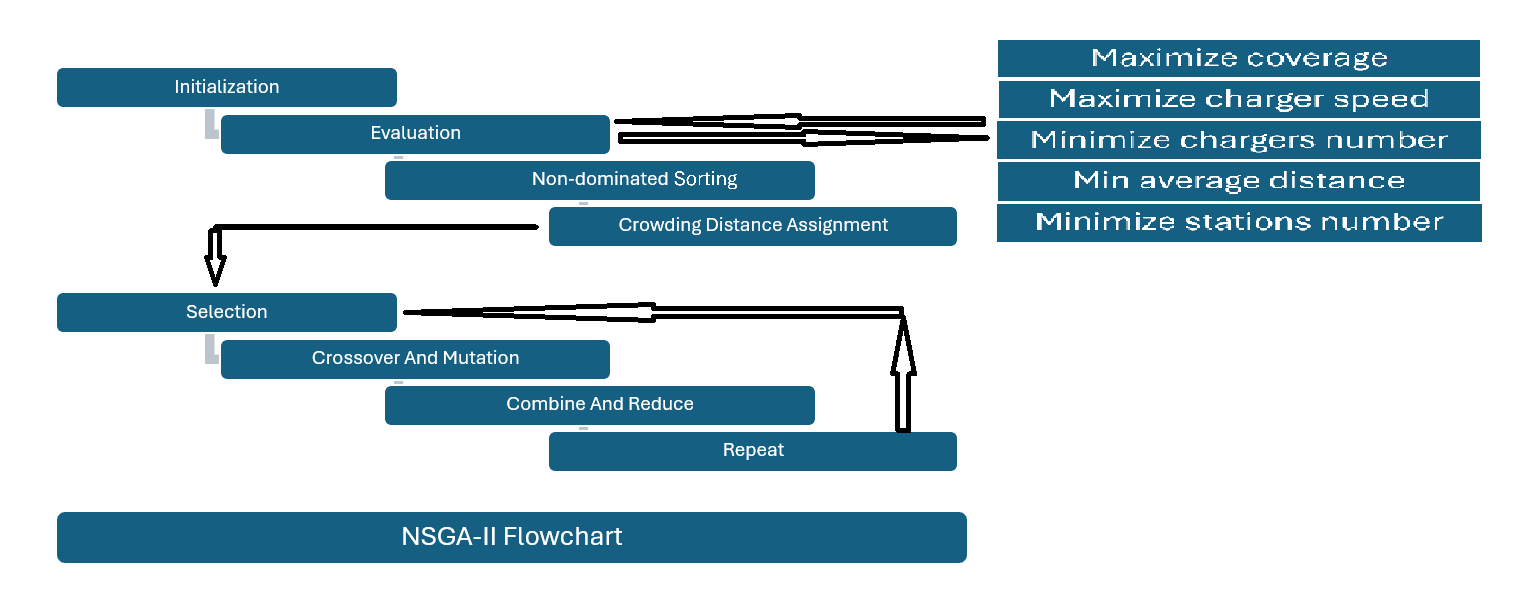
\includegraphics[width=0.8\textwidth]{../Figures/evcs-nsga-flowchart.png}
    \caption{Flowchart of the NSGA-II algorithm for EVCS network optimization.}
    \label{fig:evcs_nsga_flowchart}
\end{figure}


